%!Tex Root = ../main.tex
% ./Packete.tex
% ./Design.tex
% ./Deklarationen.tex
% ./Vorbereitung.tex
% ./Aufgabe1.tex
% ./Aufgabe2.tex
% ./Aufgabe4.tex
% ./Appendix.tex

\section{Aufgabe 3}

\setcounter{exercise}{1}

% \begin{frame}[allowframebreaks]{Aufgabe \thesection}{Zustandsdiagramme, Mealy-Automaten}
%
% \end{frame}

    % \begin{frame}{Aufgabe 3}{}
    %     \begin{block}{Aufgabe}
    %         Zeichne Zustandsdiagramm von:\\
    %         Incrementer einer Binärzahl als Mealy-Atomat:
    %         \begin{itemize}
    %             \item niedrigstwertiges Bit wird zuerst gelesen
    %             \item auf das höchstwertige Bit folgt $\#\#$
    %             \item das erste $\#$ wird durch das Überlauf-Bit ersetzt, das zweite bleibt stehen
    %             \item Symbole nach der Endmarkierung sollen durch $\#$ ersetzt werden
    %         \end{itemize}
    %     \end{block}
    % \end{frame}

    \begin{frame}{Aufgabe \thesection}{Zustandsdiagramme, Mealy-Automaten}
        \begin{solutionnoinc}
            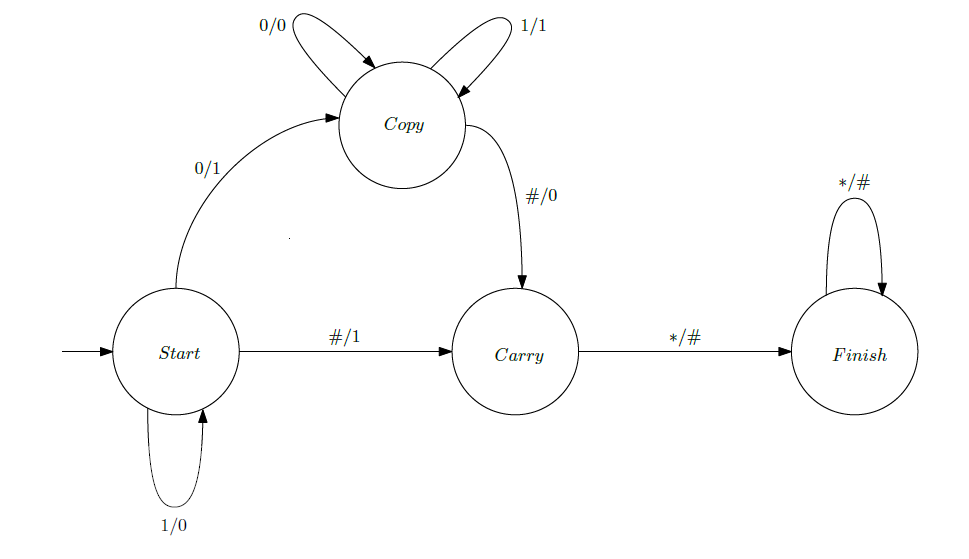
\includegraphics[height=0.5\paperheight, center]{./figures/Mealy-Increment.png}
        \end{solutionnoinc}
    \end{frame}

    \begin{frame}[allowframebreaks]{Aufgabe \thesection}{Zustandsdiagramm, Mealy-Automaten}
      \begin{solution}
        \begin{itemize}
          \item Zum Inkrementieren müssen vom niederwertigsten Bit an alle 1en in 0en verwandelt werden, bis man entweder zum Wortende oder zur ersten Null gelangt. 
          \item Im Falle einer Null, wird diese in eine Eins verwandelt und man geht in den Zustand Copy. Hier wird bis zum Wortende alles kopiert. 
          \item Liest man das erste \#, so wird das Übertragsbit ausgegeben
          \begin{itemize}
            \item Hat man schon 0en gefunden (Copy), ist das Übertragsbit 0, ansonsten 1
          \end{itemize}
        \item Dann ist man am Wortende angelangt (d. h. man liest zum zweiten Mal \#), wird an die Zahl vorne ein \# angehängt und man geht zum Endzustand
        \item Wegen Vollständigkeit muss jeder Zustand je eine Kante für jeden Eingabebuchstaben besitzten. $*$ kennzeichnet eine Kante, die für alle möglichen Eingabebuchstaben gilt
        \end{itemize}
      \end{solution}
    \end{frame}

% Vorgehen: Ein Zustand gibt an, wie weit man noch vor einem möglichen fertigen Wort entfernt ist. Man fragt sich bei jedem Zustand für alle Symbole aus Σ Σ, was es jetzt für die Entfernung zu einem fertigen Wort bedeuten würde. Z.B. bei 2 Zustände vor dem Endzustand und alle Zeichen durchgehen und nachdenken, was würde es jetzt bedeuten wenn jetzt dieses Zeichen kommt? Zu welchem Zustand würde man zurückgeworfen werden? Nicht vergessen, dass es auch Schleifen gibt! Veilleicht von den Endzuständen aus anfangen und wenn man weiß, dass es mit Sufix 110 endet diese schonmal hinschreiben.
